\documentclass[jou]{apa6}
%\documentclass[11pt]{article}
\usepackage{ucs}
\usepackage[utf8x]{inputenc}
\usepackage{changepage}
\usepackage{graphicx}
\usepackage{amsmath}
\usepackage{gensymb}
\usepackage{amssymb}
\usepackage{enumerate}
\usepackage{tabularx}
\usepackage{lipsum}
\usepackage{hyperref}

\oddsidemargin 0.0in
\evensidemargin 0.0in
\textwidth 6.27in
\headheight 1.0in
\topmargin -0.1in
\headheight 0.0in
\headsep 0.0in
\textheight 9.0in

\usepackage{xcolor}

\setlength\parindent{0pt}

\newenvironment{myenv}{\begin{adjustwidth}{0.4in}{0.4in}}{\end{adjustwidth}}
\renewcommand{\abstractname}{Anotācija}
\renewcommand\refname{Atsauces}



\newcounter{alphnum}
\newenvironment{alphlist}{\begin{list}{(\Alph{alphnum})}{\usecounter{alphnum}\setlength{\leftmargin}{2.5em}} \rm}{\end{list}}


%16.3-6

\makeatletter
\let\saved@bibitem\@bibitem
\makeatother

\usepackage{bibentry}
%\usepackage{hyperref}


\title{Homework 1: Grading Criteria}
\author{Kalvis}
\affiliation{RBS}



\begin{document}
\thispagestyle{empty}

%\twocolumn

\begin{center}
{\Large RBS: Discrete Structures}\\
{\Large RBS: Individual Presentations Part 1: Planning and Analysis}
\end{center}

{\bf Introduction:} This chart is an outline that is commonly used to develop various 
technical training. The end result is Instructional Content (also named {\em courseware}) \textendash{} 
slides, instructor demos and walk-throughs (hands-on activities that all do together), 
videos, supplementary materials for teachers, etc.\\
In this course you will use minimal planning document to prepare a $10$ minute presentation 
(desirably with a little interactive part to involve your audience) 
about an individual topic about Discrete Mathematics. 

\begin{center}
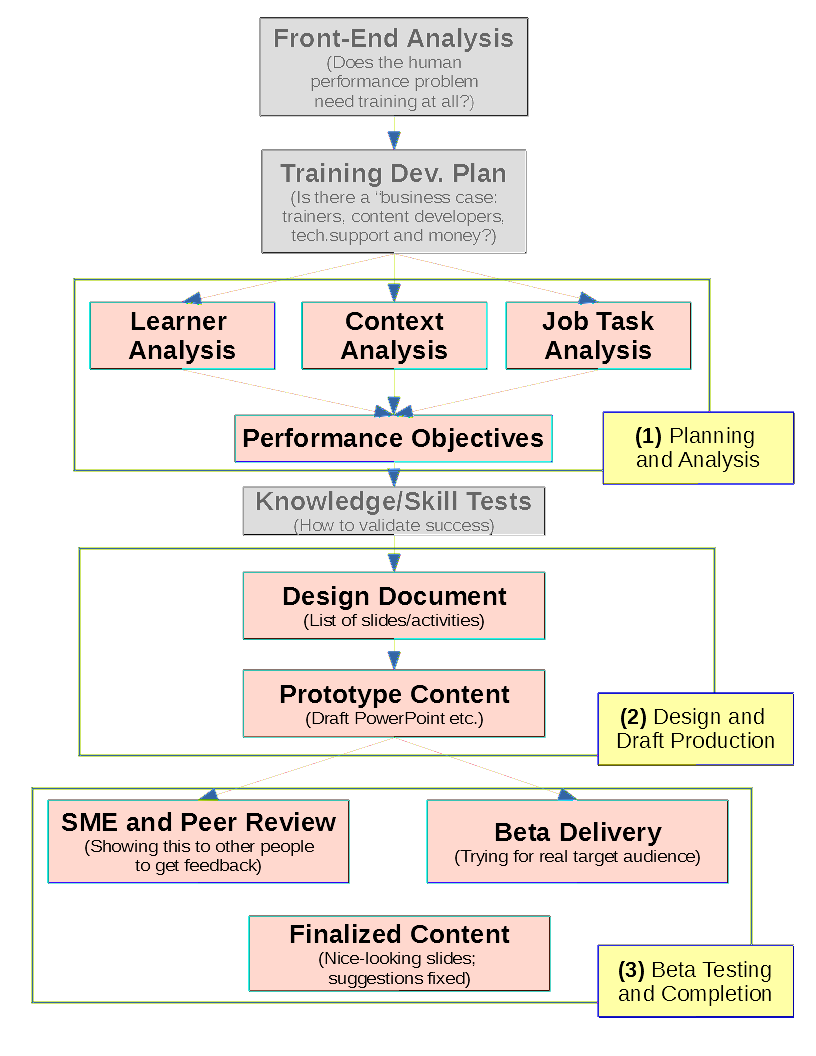
\includegraphics[width=5in]{isd-process.png}
\end{center}


The first submission is your “Planning and Analysis Document”. It is supposed 
to be 1--2 pages, but it needs to answer to a few essential questions regarding 
your upcoming presentation. By following even a very abbridged methodology 
we expect to improve your skills – how to present a technical talk (regardless of a topic). 
What is submitted in the part ``Planning and Analysis''?

Your deliverable (a LibreOffice ODT, a MS Word DOCX, or a PDF document) 
should contain $4$ sections explained below. 



\vspace{20pt}
{\large Section 1: Learner Analysis}

{\footnotesize The goal for this section is to find out the pre-existing knowledge, 
attitudes, learning preferences and tool skills of your target audience. 
Even a well-designed training may fail, if it is tailored 
for a very different audience than you actually have.}

{\bf 1.1.  Pre-existing Knowledge.} 
Try to answer at least 2 questions from the 5 questions given below – the ones that seem most relevant in your case.
\begin{enumerate}[(1)]
\item What (if anything) your audience already knows about the topic that you are going to present? 
\item Are there any people with negative experiences or issues about the topic you are going to present?
\item Could they have any misconceptions about your topic? Is there a chance to challenge those misconceptions?
\item Could there be problems with how they understand some special terminology, language or examples you are going to use? 
\item Does your topic relate to anything else they had been doing or experiencing (perhaps, other university courses or work life).
\end{enumerate}

{\bf 1.2. Pre-existing Attitudes.} Try to answer both questions given below.
\begin{enumerate}[(1)]
\item Any part of your topic to which your audience could have 
positive feelings \textendash{} benevolent understanding, curiosity, joy.
\item Any part of your topic to which your audience could have 
negative feelings that could interfere in the training.
\end{enumerate}

{\bf 1.3. Language Preferences.} Try to answer both questions given below.
\begin{enumerate}[(1)]
\item Knowledge of the special terms that you are going to use?
\item Which language style would work better for your topic \textendash{} 
does it need to be technical, conversational/informal, mixed? 
Does your audience have sensibilities regarding your style? 
\end{enumerate}
Some audiences may dislike sexist jokes, strange cultural references, etc. 
Is there anything that you want to avoid in front of this audience?

{\bf 1.4. Tool and Method Preferences.} Try to answer both questions given below.
\begin{enumerate}[(1)]
\item Training delivery method likes and dislikes (in your case it could be – projector vs. paper handouts vs. flipcharts vs. answering your questions vs. using their phones to enter Mentimeter, etc.)
\item Do they need to know, how to use some tool befor your class?
\end{enumerate}


\vspace{20pt}
{\large  Section 2: Context Analysis} 

{\footnotesize Try to keep this section short, but relevant!}

The goal of this section is to describe the environment; the circumstances \textendash{} 
how this training will occur. Most likely the answers to most of these questions is obvious, 
but you might need to clarify some of the topics.

Try to answer at least 4 questions from the 12 questions given below – the ones that seem most relevant in your case.

\begin{enumerate}[(1)]
\item Is the delivery of your topic necessarily instructor-based 
(i.e. the training will need you – or some other human as a teacher)? 
Or can it be fully or partly automated (as in a video-lecture, 
KhanAcademy or MOOC course delivery)?
\item Are there any concerns about your qualification as an instructor 
(is there a substantial knowledge gap; or even a need to change your topic?)
\item Which room would you prefer for the delivery, what table arrangment would you need? 
\item How does your topic relate to other topics in the Discrete Structures course? 
(Do you need to speak BEFORE or AFTER some other student? Or, perhaps, 
do you need the instructor to cover some topic as a prerequisite?)
\item Do you need some technical or other assistance during the course delivery?
\item Do you need any specific harware or software tools to be available 
(multimedia projector? whiteboard? HDMI, VGA video-ports to connect your laptop? loudspeakers?)
\item Is there some “external motivation” for the audience – WHY would they pay attention to what you are telling?
\item Do you gather any feedback, tests etc. to see what they have learned?
\item Do you check the attendance? 
\item Can you estimate, how much of your time you can afford to spend to prepare this stuff? 
(There may be other courses, deadlines, family commitments, etc.)
\item Any other time limits or scheduling constraints?
\item Are there any legal concerns that are relevant? Properly attributing authorship 
for copyrighted material or stock photos in your presentations?  
\end{enumerate}



\vspace{20pt}
{\large Section 3: Job Task Analysis}

{\footnotesize Create a list of some 3-8 ``job tasks''.}

In this section you can list specific knowledge and skills that the audience 
will gain from youur presentation. It is usually called “job” task analysis \textendash{} 
because the skills are assumed to be relevant for somebody who is doing their day-to-day job. 
There can be two types of knowledge:

\begin{itemize}
\item ``procedural knowledge'' (people will learn steps, how to do something specific).
\item ``conceptual knowledge'' (people will learn about some qualities, new terminology and examples). 
\end{itemize}

JTA is usually presented as a hierarchy of tasks:
Ideally, you should come up with a “Tree-view” of the tasks. There is one ``root task''
(e.g. ``Identify and compare algorithms ... and ...'') with 2--7 appropriate subtasks. 
For short presentations you probably do not need multi-level hierarchy.

There are many examples in the Internet, how to do JTA (job task analysis).\\
For Discrete mathematics topics see \url{https://bit.ly/3d8AnYE}.\\
For high-school number theory see \url{https://bit.ly/2vxCWTa}.\\
In all cases it is essential to express each skill in a single sentence; and that sentence should start with a short verb. 

\begin{quote}
Examples of verbs you can use include (but are not limited to):\\
{\em “choose...” , “complete...”, “define...”, “detect...”, “distinguish...”, 
“identify...”, “label...”, “list...”, “match...”, “order...”, “select...”,  
“classify...”, “find...”, “formulate...”, “quote...”, “suggest...”.}

Some verbs may be specific mathematic manipulations:\\
{\em “add...”, “bisect...”, “calculate...”, “check...”, “compute...”, “count...”, “derive...”, “divide...”, “estimate...”, “measure...”, “multiply...”, “prove...”, “subtract...”.}
\end{quote}

It is sometimes relevant, which verb you use. Consider examples:
(1) “LIST all five great lakes” means ability of the trainee to say aloud “Huron, Ontario, Michigan, Erie, Superior” (then you teach mnemonic HOMES). 
(2) “MATCH five great lakes with regions in an unlabeled map” means the ability to locate them on a map. 
(3) “IDENTIFY the great lakes among the others” means the ability to distinguish them from distractors (for example, other lakes that are not great).



\vspace{20pt}
{\large Section 4: Performance Objectives}

Rewrite your tasks from Section 3 as 3--8 objectives.

At this stage you take every task/skill from the previous section and describe, 
what story or activity is going to address it. You formulate the 
specific context, where that task/skill is embedded and will happen.

For example, if your task from Section 3 is 
{\em ``Understand and Use the Vieta's formulas for quadratic equations''}
then objective in Section 4 would be slightly longer. For example:

\begin{quote}
Given a quadratic equation with small integer-valued roots, the learner can tell the 
sum $x_1+x_2$ and the product $x_1 \cdot x_2$ of its roots; 
and can factorize it as $a(x - x_1)(x - x_2)$.
\end{quote}




\section{Bibliography}

\begin{enumerate}
\item Neal Ford. Presentation Patterns: Techniques for Crafting Better Presentations. Pearson Education, 2012.
\item Harold D. Stolovitch, Erica J. Keeps. Telling ain’t Training, 2nd Edition.  Association for Talent Development; 2011. 
\item Harold D. Stolovitch. Training ain’t Performance.  Association for Talent Development; 2006.
\end{enumerate}



\end{document}



